\begin{frame}[hasprev=false, hasnext=true]
\frametitle{McCabe example}
\label{example:mccabe}

Consider the graph below:

\begin{figure}
	\centering
	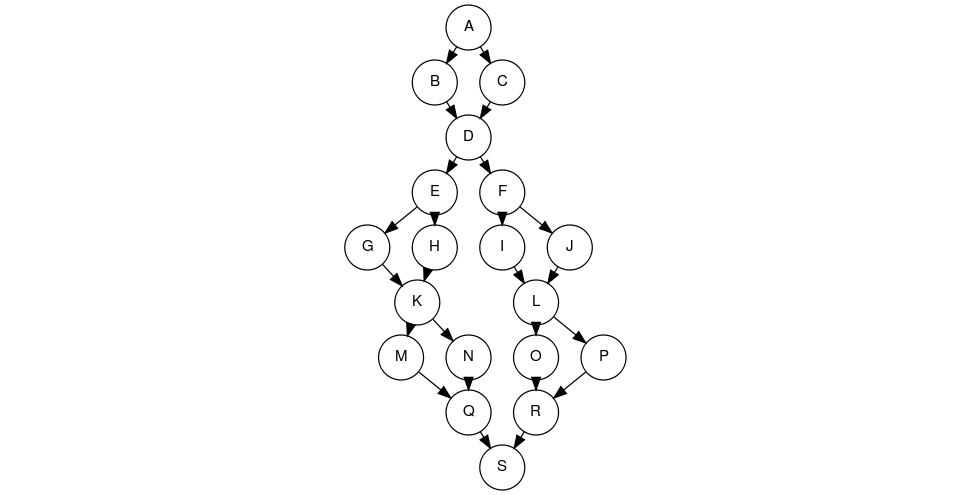
\includegraphics[scale=.3]{aux/examples/mccabe/mccabe-example}
\end{figure}

The cyclomatic complexity of the graph is 7. So, seven test requirements,
thus seven complete paths, must be devised for the graph.
\end{frame}


\begin{frame}[c, hasprev=true, hasnext=true]
\frametitle{McCabe example}
\framesubtitle{Path 1}

\begin{figure}
	\centering
	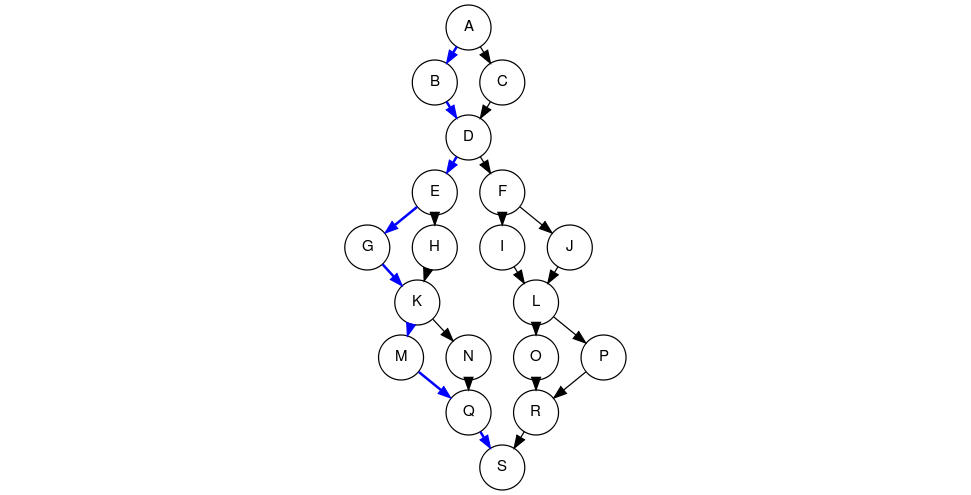
\includegraphics[scale=.3]{aux/examples/mccabe/mccabe-example-path-1}
\end{figure}
\end{frame}


\begin{frame}[c]
\frametitle{McCabe example}
\framesubtitle{Path 2}

\begin{figure}
	\centering
	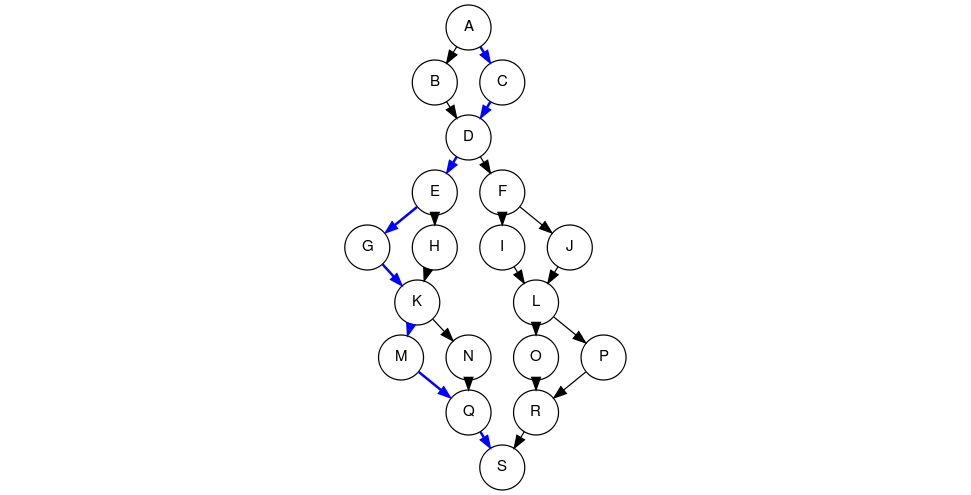
\includegraphics[scale=.3]{aux/examples/mccabe/mccabe-example-path-2}
\end{figure}
\end{frame}


\begin{frame}[c]
\frametitle{McCabe example}
\framesubtitle{Path 3}

\begin{figure}
	\centering
	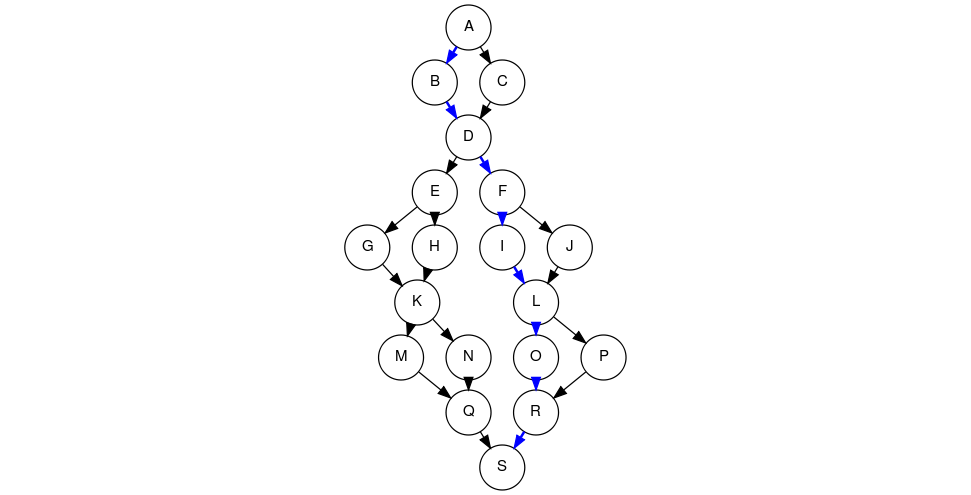
\includegraphics[scale=.3]{aux/examples/mccabe/mccabe-example-path-3}
\end{figure}
\end{frame}


\begin{frame}[c]
\frametitle{McCabe example}
\framesubtitle{Path 4}

\begin{figure}
	\centering
	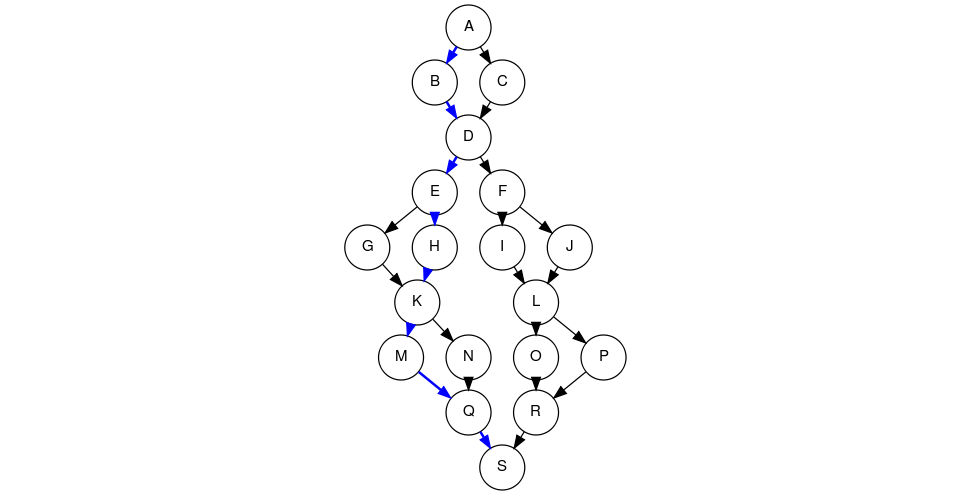
\includegraphics[scale=.3]{aux/examples/mccabe/mccabe-example-path-4}
\end{figure}
\end{frame}


\begin{frame}[c]
\frametitle{McCabe example}
\framesubtitle{Path 5}

\begin{figure}
	\centering
	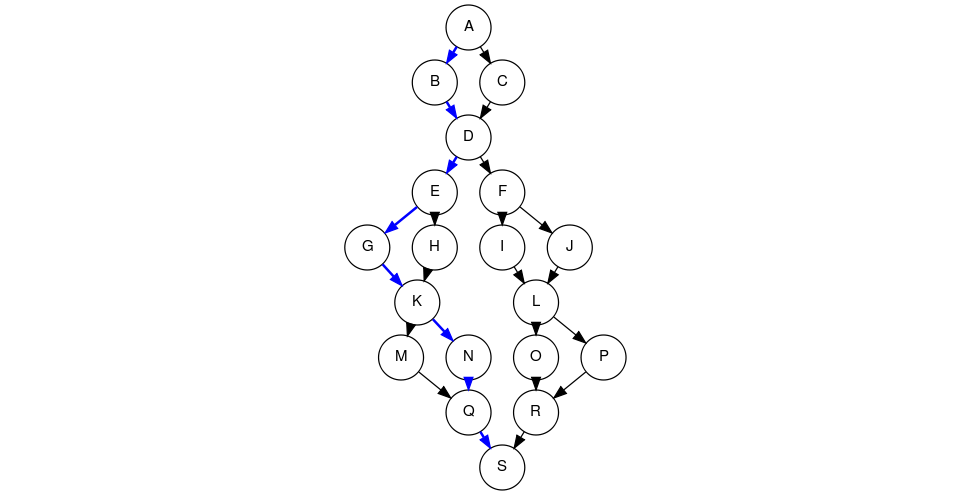
\includegraphics[scale=.3]{aux/examples/mccabe/mccabe-example-path-5}
\end{figure}
\end{frame}


\begin{frame}[c]
\frametitle{McCabe example}
\framesubtitle{Path 6}

\begin{figure}
	\centering
	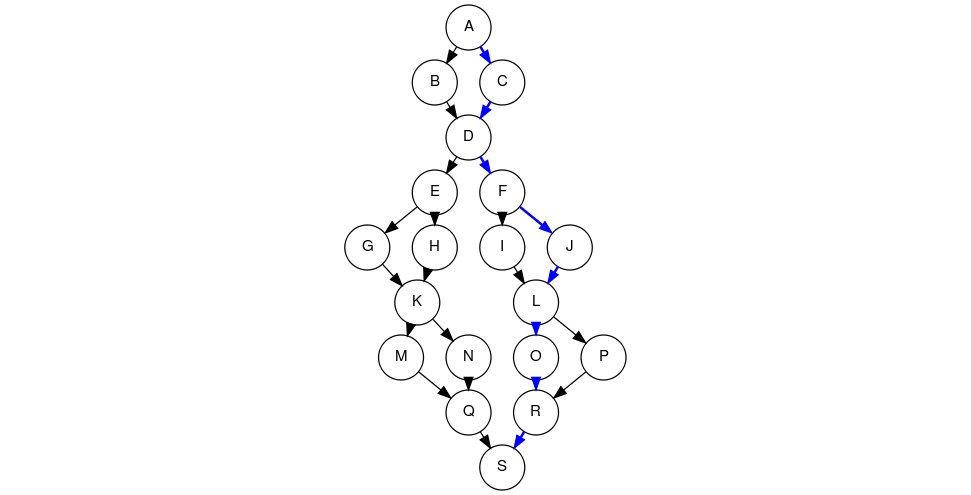
\includegraphics[scale=.3]{aux/examples/mccabe/mccabe-example-path-6}
\end{figure}
\end{frame}


\begin{frame}[c, hasprev=true, hasnext=false]
\frametitle{McCabe example}
\framesubtitle{Path 7}

\begin{figure}
	\centering
	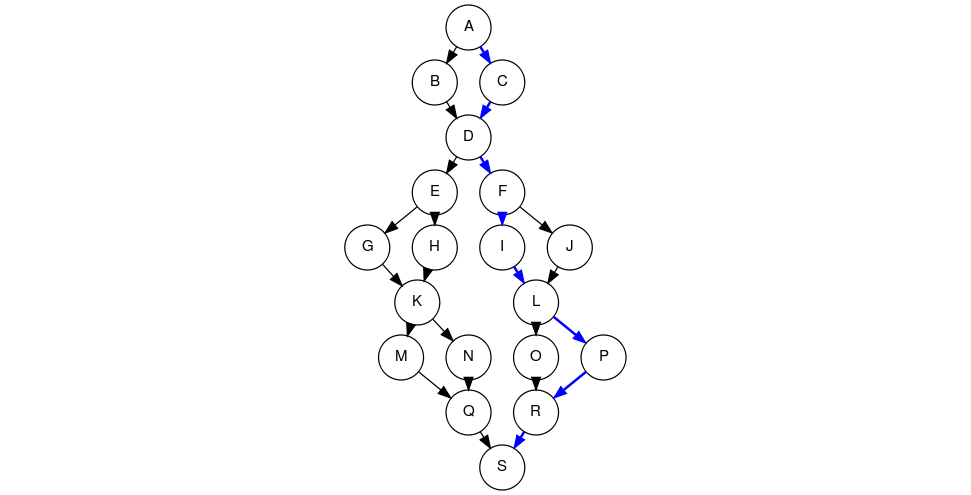
\includegraphics[scale=.3]{aux/examples/mccabe/mccabe-example-path-7}
\end{figure}
\end{frame}